\section{Advert Server Design}
\label{serverdesign}
Below we will describe some high-level design decisions we made, prior to
implementing our application storage server at the Google App Engine.

\subsection{Server Structure}
\label{server-design-structure}
The application storage server will have an iterative structure, where clients
are served on a one-thread-per-client basis; it will receive a client request,
process it and return a reply (all in HTTP as described below). Since the App
Engine distributes each request to possibly a different server, concurrency can
occur, so a form of synchronization is needed (see Section
\ref{serverdesign-transactions}).

\subsection{Client Functions}
The server provides some generic functions as an interface to its clients. These
functions are derived from the \emph{JavaGAT AdvertService} \cite{javagat-www}. 
Below is an overview of which functions are going to be implemented.

\begin{itemize}
	\item \texttt{void add(object, metadata, path)}; Add an object with meta data to
		the datastore
	\item \texttt{Object get(path)}; Gets an object from the datastore
	\item \texttt{void delete(path)}; Delete an object from the datastore
	\item \texttt{MetaData getMetaData(path)}; Gets meta data from the datastore
	\item \texttt{String[] find(metadata)}; Query the service for entries matching
		a specified set of meta data 
\end{itemize}

Note that not all functions provided by the JavaGAT AdvertService, are
implemented, but only the most useful and necessary functions will be
available. This way, we offer a more generic Advert server which might be
used for other purposes than an AdvertService Adaptor (e.g. see Section
\ref{ipl}).

% \subsubsection{Functions to Implement} 
% Looking at the javadoc of the JavaGAT \cite{javagat-javadoc}(the AdvertService in
% specific), there are some basic functions we can implement using the App Engine.
% First of all a very important function is the function called
% \texttt{marshall()}, which takes a random object (stream of bytes) and creates a
% String representation of this object. This object can then be used by the
% following functions:
%
% A good example are the \texttt{getPWD()} and \texttt{setPWD()} functions. Both
% functions are necessary to make the AdvertService adapter for the Google App
% Engine. However, these functions won't be very helpful for the other uses of our
% service. That's why they won't be implemented into our library (which
% communicates with the App Engine), but they will be in the adapter (locally).

\subsection{Datastore Layout}
The App Engine scalable datastore stores and performs queries over data objects,
known as entities. An entity has one or more properties, named values of one of
several supported data types. A property can be a reference to another entity, to
create one-to-many or many-to-many relationships. Below we will describe which
datatypes we designed for the datastore.

\subsubsection{Data Types}
From our user functions as specified above, we can specify our data types,
needed to store the Advert objects with associated meta data.

\paragraph{Advert Object}
In general, Advert object are structured as shown in Figure
\ref{serverdesign-advert-obj}. Objects added to the datastore are stored as
unicode text, which is a decision we made over time. Although the Google App
Engine supports a so called \emph{BlobProperty} for storing binary data, it is
more useful to store objects as unicode text, as we will see in Section
\ref{serverdesign-transfer-protocol}.

Additionally, a path name is added, in order to identify the object. Also a
username and a \emph{TTL} (Time To Live, see Section \ref{serverdesign-ttl}) is
added to each Advert object stored in the datastore.

\begin{figure*}[ht] %[placement] where placement is h,t,b,p
\begin{center}
\begin{code}
class Advert(db.Model):
  path   = db.StringProperty()
  author = db.UserProperty()
  ttl    = db.DateTimeProperty(auto_now_add=True)
  object = db.TextProperty() 
\end{code}
\caption{The Layout of an Advert Object.\label{serverdesign-advert-obj}}
\end{center}
\end{figure*}

\paragraph{Meta Data Object}
In addition to storing the Advert object, meta data may be specified to be
stored along with the object. Meta data consists out of a set of key-value
pairs, which describe the data. Unfortunately, the Google App Engine does not
support tuples or something similar to tuples, so we created our own meta data
object as shown in Figure \ref{serverdesign-metadata-obj}.

\begin{figure*}[ht] %[placement] where placement is h,t,b,p
\begin{center}
\begin{code}
class MetaData(db.Model):
  path   = db.StringProperty()
  keystr = db.StringProperty()
  value  = db.StringProperty()
\end{code}
\caption{The Layout of a Meta Data Object.\label{serverdesign-metadata-obj}}
\end{center}
\end{figure*}

We had various options in implementing the meta data object. We tried to make
an array of a custom key-value pair objects, which did not work in Python. We
also thought of saving all key-value pairs in a long delimited String, but this
solution does not make the meta data objects searchable. The most obvious
solution is to store every key-value pair seperately in the datastore and add
an identifier to them (in this case the pathname), to group them together
eventually.
 
\subsubsection{Garbage Collection}
Since the capacity of the datastore is limited to 1\,GB, we need some sort of
\emph{garbage collection} to keep our service usable for storing new data. This
is only possible by overwriting old data with new data (i.e. removing non-used
items to make room for new data). Removing old items is called garbage
collection.

\paragraph{TTL}
Initially we will give each data item stored in the server a Time To Live (TTL)
value. This TTL has a fixed value (we chose 10 days), after which the data will
be removed from the datastore, making room for new data. Alternatively, we could
give data items a dynamic value for their TTL, depending on the usage of the
datastore (i.e. if the datastore is almost full, we will give data a shorter
TTL). We did not choose to implement the latter option because this way we
cannot guarantee the time an object is present in the datastore. By setting the
TTL to a fixed amount of time, we can guarantee that a data item is in the
datastore for at least that fixed amount of time, and maybe, if the user is
lucky, even longer.

\paragraph{FIFO and LRU}
Secondly, if we would not give a TTL value to each data item stored in the
datastore, we could remove the oldest item as soon as we run out of free storage
space. By giving all items a timestamp as soon as we store then in the datastore,
we could find the oldest and remove it from the datastore to make room for new
data. Also we could make something like a LRU list (Least Recently Used), after
which we update the timestamp as soon as a data item was referenced or edited.
This way, only the data items that are least referenced are deleted, as soon as
we run out of storage. A disadvantage of this scheme is that this could lead to
clients referencing them only the keep them alive in the datastore, and
unnecessarily using bandwidth as a consequence. Our main purpose for the TTL is
to prevent clients from storing data in the datastore and forgetting to delete it
(which would result in an overfull datastore).

\paragraph{Frequency}
Once every request (or once every x requests), we could query the datastore for
expired items and delete them from the datastore accordingly. Another option
would be to remove the items which are expired as soon as we run out of free
storage space. We chose to implement the latter, becuase this gives less
overhead than starting a garbage collector every request. When the datastore is
full and there is no data to be evicted, we return an error to the client, which
throws an \texttt{AppEngineResourcesException}. The client can then try again at
a later moment in time, or use another server.

\subsubsection{GQL Queries}
Google provides us with the \emph{Google Query Language} (GQL), which is similar
to \emph{SQL} (Structured Query Language). An example GQL query is shown in
Figure \ref{serverdesign-gql-example}. These queries are powerful for searching and
retrieving objects from the datastore. 

\begin{figure*}[ht] %[placement] where placement is h,t,b,p
\begin{center}
\begin{code}
db.GqlQuery("SELECT * FROM MyModel WHERE s1 >= :1 AND s2 < :2", "foo", "bar")
\end{code}
\caption{GQL Query example.\label{serverdesign-gql-example}}
\end{center}
\end{figure*}

SQL queries are generally vulnerable to SQL injection,
which is a technique that exploits a security vulnerability occurring in the
database layer of an application. Basically it would make it possible to insert
an SQL statement within a statement, and execute custom code. Usually this
custom code exists of malicious statements like \texttt{DROP}. Since the Google
App Engine's GQL Syntax only supports the \texttt{SELECT} stament, we do not
have to prevent this (see Figure \ref{serverdesign-gql-syntax}).

\begin{figure*}[ht] %[placement] where placement is h,t,b,p
\begin{center}
\begin{code}
  SELECT * FROM <kind>
    [WHERE <condition> [AND <condition> ...]]
    [ORDER BY <property> [ASC | DESC] [, <property> [ASC | DESC] ...]]
    [LIMIT [<offset>,]<count>]
    [OFFSET <offset>]

  <condition> := <property> {< | <= | > | >= | = | != } <value>
  <condition> := <property> IN <list>
  <condition> := ANCESTOR IS <entity or key>
\end{code}
\caption{GQL Syntax.\label{serverdesign-gql-syntax}}
\end{center}
\end{figure*}

In addition, the App Engine does not support multiple queries seperated by a
semi-colon (``\texttt{;}''), because it raises a parse error. Only one query at
a time can be executed and there is no support for nested queries also.

\subsubsection{Concurrency Control}
\label{serverdesign-transactions}
The datastore uses \emph{optimistic locking}\footnote{Optimistic locking (also
known as optimistic concurrency control) is based on the assumption that most
database transactions don't conflict with other transactions.} for concurrency
control. An update of an entity occurs in a transaction that is retried a fixed
number of times if other processes are trying to update the same entity
simultaneously. Our application can execute multiple datastore operations in a
single transaction, which either all succeed or all fail, ensuring the integrity
of data. 

\subsection{Transfer Protocol}
\label{serverdesign-transfer-protocol}
Since the Google App Engine only offers functions in a sandbox, as stated above,
it is not possible to make connections to the App Engine, other than using HTTP
or HTTPS. Furthermore, once a HTTP request is issued, a response is expected within
a few seconds, otherwise the connection times out. To implement the functions
specified above we designed our own protocol of sending and receiving data to
and from the Google App Engine.

\subsubsection{HTTP Requests}
Google offers an URL Fetch function, which supports five HTTP methods: GET, POST,
HEAD, PUT and DELETE. For the functions described below, it would be useful to
have an HTTP method that would allow us to send some (binary) data (i.e. POST or
GET), after which we do not only get a success return value; but also data as a
return value. This would be especially useful for the \texttt{find()} function.
The HTTP POST function servers our needs best, since the GET function translates
all data into a URL formatted String (which would be inappropriate for binary
data). Secondly, according to the HTTP RFC , the default HTTP response is a
status line (e.g. ``200 OK''), followed by a message body. This suits the needs
for the implementation of our server.

\subsubsection{Object Encoding} 
Since we are sending multiple data items over a single HTTP connection we will
encode all data so it will be transferred in one HTTP request. It is necessary
to transfer all data in one HTTP request to avoid inconsistencies in the
datastore. To achieve this we came up with multiple schemes to encode all data
in a single HTTP request, as is shown below.

\paragraph{Multipart/Form-Data}
HTTP natively supports a standard for sending a combination of both URL encoded
Strings and binary data. This is specified in \emph{RFC1867} as
\emph{multipart/form-data}. Although this would seem perfect for our purposes, we
decided not to use this standard for sending a combination of URL encoded Strings
and binary data. RFC1867 specifies that every part of the message should be
seperated by a boundary, chosen by the client. The downside is that this boundary
cannot appear in the content of the payload. Since our payload can be virtually
anything, we decided to go in a different direction, because otherwise we would
have to perform a linear search on all our data to see if a boundary token would
accidentally appear in our payload.

\paragraph{Custom Scheme}
Instead of using boundaries to define the start/end of our payload, we could make
use of special bytes which define the length of our payload. The layout of this
scheme is shown in Figure \ref{clientimpl-custom}. To begin with we start by
sending the length of the path, which is our first four bytes. Now the server
knows how many bytes the path will be (which is variable n), after which it knows
the meta data will follow. The meta data also starts with four bytes, indicating
the length (variable m). Finally, the object is sent, again, by sending the
object length as the first four bytes and the object (variable size p) right
after that.

\begin{figure*}[ht] %[placement] where placement is h,t,b,p
\begin{center}
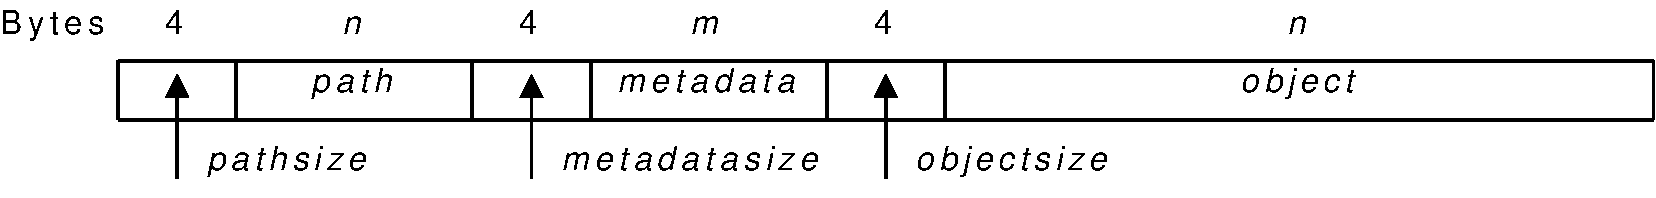
\includegraphics[width=12cm]{./figures/custom_payload.pdf} 
\caption{Custom Payload for Sending Binary Data.\label{clientimpl-custom}}
\end{center}
\end{figure*}

Our first attempt of sending the meta data was to structure it like this:
key1=value1: key2=value2: key3=value3: etc. At the client side, we would have to
escape actual content containing the equals sign or a colon, by placing a
backslash in front of them. We had to decode this again at the server side, to
make successful searches. To encode key-value pairs we could make use of
\emph{JSON} (JavaScript Object Notation) \cite{json-www}. JSON is designed --
hence very effective -- for encoding such key-value pairs into serial forms.
Below we take this even further, since JSON can encode more than just
key-value pairs.

\paragraph{JSON}
Besides serializing meta data object, JSON can actually serialize our whole
payload for us. This means that we don't have to work with neither boundaries,
as used in multipart/from-data, nor with payload sizes. Since both Java and
Python can use libraries which implement all JSON functionality, we will not
have to program a new mechanism of sending multiple Strings and binary data
in one request. 

To give the reader a small idea of how JSON works, we will try to encode te
payload above into a serial JSON String. The message consists out of three parts:
a path, meta data, and a binary object. So we will make a JSON array, with each
entry containing a part. The first part is just a String, which is a value for
the first entry. The second part is something more complicated, which we will
encode as a JSON obect, storing key-value pairs. The third entry again is a bit
more difficult, since we can only store Strings, numbers, booleans, and null.
That's why we formatted the binary object into a \emph{Base64} encoded
String\footnote{Base64 refers to a specific MIME content transfer encoding. It
encodes binary data by treating it numerically and translating it into a base 64
representation.}. The only downside is that Base64 encoding has a overhead of
about 1.35 of the original data length. For more information about the JSON
format, we refer to \cite{json-www}.

Once encoded, we can serialize the JSON array to a String (see Figure
\ref{clientimpl-json}), after which it will be sent to the server. We can decode
this String using simplejson at the server side, retrieving our JSON array back
(see Section \ref{serverimpl-simplejson}). 

\begin{figure*}[ht] %[placement] where placement is h,t,b,p
\begin{center}
\begin{code}
["/home/bboterm/app-engine/",{"key1":"value1","key2":"value2","key3":"value3"},
  "R0lGODlh(...)KSAAOw=="]
\end{code}
\caption{An example of a serial JSON array.\label{clientimpl-json}}
\end{center}
\end{figure*}

% 
% Our Java Adaptors could easily use these methods to authenticate themselves (with
% or without Google Accounts), and call functions, possible sending data as
% parameter of a function (using \emph{SOAP}\footnote{SOAP stands for Simple
% Object Access Protocol, a protocol specification for exchanging structured
% information in the implementation of Web Services. \cite{soap-www}} or
% \emph{JSON} (JavaScript Object Notation) \cite{json-www} for example).
% 
% For Python \emph{simplejson} \cite{simplejson-www} is available, which is a
% simple, fast, complete, correct and extensible JSON encoder and decoder for
% Python 2.4+. It is pure Python code with no dependencies, but includes an
% optional C extension for a serious speed boost. From Python 2.6, JSON is
% contained in the standard library, but since Google makes use of Python version
% 2.5.2, it is likely that simplejson is needed.
% 
 
\subsection{Authentication and Privacy}
Google provides two forms of authentication with its App Engine.

\begin{itemize}
\item By means of a \emph{Google Accounts} (also used for Gmail, iGoogle, etc)
\item Google Apps for your Domain
\end{itemize}

For the first option, Google's unified sign-in system is used. All a user needs
is a valid email address (it doesn't need to be a Gmail address!) to sign up for
a Google Account. For the second option, users of Google Apps for your Domain can
choose to restrict all or part of their web application to only those people who
have a valid email address on their domain.

\subsubsection{Authentication through Google Accounts}
For our purposes it would be most attractive to make use of the authentication
through Google Accounts. An application can redirect a user to a Google Accounts
page to sign in or register for an account, or sign out; using simple functions
like \texttt{create\_login\_url()}. After a successful login session the
application can retrieve a User object to authenticate a user.

% If one is to log in manually (\texttt{create\_login\_url()} was called), one
% would see a login page, similar to that of other Google services, like Gmail for
% example. Once one has pushed the `Sign in' button, username and password are sent
% over HTTPS, after which a cookie is stored at the user side, containing a session
% ID (ACSID). This cookie is used for all sessions until logout is initiated.

\subsubsection{Own Authentication Scheme}
Second possibility would be to drop the concept of Google Account authentication,
and write our own authentication scheme (for example using a private-public key
pair). This has the advantage that we could apply a much more sophisticated
authentication scheme and give more guarantees with respect to the issues stated
above. A disadvantage is that it takes a lot more time and knowledge to implement
your own authentication scheme, while there is a perfectly fine solution at hand
(i.e. Google Accounts).

Note that both solutions do not necessarily implement hierarchy in users. There
will be an interface for the administrator, but that stands aside of the service
we are offering (this interface is offered by the Google App Engine). Otherwise
it seems logical to use the Google Accounts for authentication (if we want to run
a `private' service), since its much more efficient and less time-consuming than
inventing our own authentication scheme.

% Another way of not using the authentication through Google accounts would be to
% use the Django  framework, which is also supported by the Google Apps Engine.
% Various examples of this authentication scheme exist.

\subsubsection{Server Authentication}
Both authentication schemes give us two options for server setups.

\begin{itemize}
  \item \textbf{Everyone Runs Its Own Service}; This way one could only
  authenticate himself by using a Google Account (i.e. one Google Account per
  organization), or restrict the application for only the domain of the
  organization using this service, or even to oneself. This way one would run out
  of resources less quickly than if one would use a (global) public service.
  Also, it is more reliable than using a public service; there is less chance of
  people reading and/or editing data stored by the service.
  \item \textbf{One Public Service for Everyone}; This way we would run an open
  service, accessible for everyone, without the need for a Google Account to
  authenticate oneself. A possible downside of this is that everyone can
  read/edit everyone's information. Also global public use might make the service
  run out of resources fast. Thus, for one global public service we can't give
  many guarantees.
\end{itemize}

We decided to implement two different servers; one without any form of
authentication (i.e. a public server), and one with authentication (i.e. only the
owner is able to use it, and additional users can be added after the server is
deployed). The user itself can choose which version of the server to install,
according to his personal needs.

\subsubsection{(In)Secure Connections}
Google provides the means of having both insecure connections (HTTP, port 80), as
having secure connections (HTTPS, port 443). Naturally some data we would rather
not share in the open (for example passwords), so that would be a use for HTTPS.
The question is, if it would be wise (and necessary) to run all traffic over
HTTPS. We have to keep in mind that our bandwidth for HTTPS is limited, but is
still a reasonable amount (see Section \ref{appengine-quotas}). Plus we don't
give any guarantees. If we run out of HTTPS, we just have to wait another 24
hours and it will work again. Either way configuration is done beforehand, when
it comes to secure connections.
